% ---------------------------------------------------------------------------
% Capítulo 2 — Marco teórico
% ---------------------------------------------------------------------------
% Redactado en tercera persona (norma 2.4). Los acrónimos se explican en su
% primera aparición dentro de este capítulo, con su traducción cuando proceden
% de otro idioma. Decimales con coma y unidades del Sistema Internacional.
% Mínimo dos páginas por capítulo (norma 2.6).

\chapter{Marco teórico}

Este capítulo reúne los fundamentos sobre los que se apoya el desarrollo. Avanza
desde el dispositivo hacia el sistema de generación: primero se describen el
microcontrolador y la cadena de herramientas que producen el código objetivo,
después los modelos de lenguaje capaces de escribirlo, la técnica de
recuperación que les aporta el conocimiento específico del dispositivo, el
protocolo con que ese conocimiento se les expone y, por último, los criterios
con que se mide el resultado.

% ===========================================================================
\section{Microcontroladores de 8 bits y la familia PIC18-Q10}
% ===========================================================================

Un microcontrolador integra en un solo circuito el procesador, la memoria y los
periféricos necesarios para gobernar un sistema empotrado. Frente a un
procesador de propósito general, sacrifica capacidad de cómputo a cambio de
determinismo temporal, bajo consumo y coste reducido, lo que lo hace idóneo para
tareas de control en tiempo real.

El dispositivo objetivo de este trabajo es el PIC18F47Q10 de Microchip
Technology, un microcontrolador de 8 bits de la familia PIC18-Q10
\cite{microchip2024ds40002043}.

\subsection{Arquitectura del núcleo}

El núcleo sigue una arquitectura Harvard modificada con juego de instrucciones
reducido: la memoria de programa y la de datos ocupan espacios separados, con
buses independientes y anchuras distintas —16 bits para las instrucciones y
8 bits para los datos—. Esa separación permite solapar la búsqueda de una
instrucción con la ejecución de la anterior.

El repertorio consta de 75 instrucciones, ampliables a 83 si se habilita el
juego extendido. La frecuencia de trabajo llega hasta 64\,MHz, con un ciclo de
instrucción mínimo de 62,5\,ns, ya que cada ciclo abarca cuatro períodos del
oscilador. El contador de programa es de 21 bits, de modo que direcciona un
espacio de 2\,MB aunque el dispositivo no lo implemente por completo.

La pila de retorno admite 31 niveles y reside en un panel de memoria estática
independiente, fuera de los espacios de programa y de datos. Es accesible por
software, lo que permite implementar mecanismos de conmutación de contexto, pero
su desbordamiento provoca un reinicio del dispositivo si así lo determina el bit
de configuración correspondiente. Las interrupciones admiten dos niveles de
prioridad programables.

\subsection{Ciclo de instrucción y segmentación}

Cada ciclo de instrucción abarca cuatro períodos del oscilador, denominados Q1 a
Q4. La búsqueda del código de operación ocupa uno de ellos y la ejecución los
restantes, de modo que el núcleo solapa la búsqueda de la instrucción siguiente
con la ejecución de la actual. En régimen permanente se completa una instrucción
por ciclo.

La segmentación se rompe cuando el flujo cambia. Las instrucciones de salto y
las condicionales cuya condición se cumple invalidan la instrucción ya buscada,
que se sustituye por una operación nula, y consumen dos ciclos. Las cuatro
instrucciones que ocupan dos palabras de memoria consumen igualmente dos ciclos.
Esta irregularidad es la razón por la que el conteo de ciclos de una rutina no
coincide con el número de instrucciones que la componen, dato relevante cuando
se generan rutinas de temporización por software.

\subsection{Organización de la memoria}

La memoria de datos se direcciona con 12 bits y se organiza en dieciséis bancos
de 256 bytes. Como la mayoría de las instrucciones solo codifica los 8 bits
menos significativos de la dirección, los 4 restantes proceden del registro de
selección de banco. Este esquema introduce una fuente de error característica de
la arquitectura: operar sobre el banco equivocado escribe en una dirección
distinta de la prevista, y el registro de estado se actualiza como si la
operación hubiera tenido éxito.

Para atenuarlo, la arquitectura reserva un espacio de acceso rápido de
256 bytes, accesible en un solo ciclo sin necesidad de fijar el banco. Lo
componen los 96 bytes bajos del banco 0, destinados a variables de uso
frecuente, y los 160 bytes altos del banco 15, donde residen los registros de
función especial más utilizados.

La tabla \ref{tab:memoria47q10} resume las capacidades del dispositivo.

\begin{table}[H]
  \centering
  \caption{Recursos de memoria del PIC18F47Q10 \cite{microchip2024ds40002043}}
  \label{tab:memoria47q10}
  \begin{tabular}{@{}lrl@{}}
    \toprule
    \textbf{Recurso} & \textbf{Capacidad} & \textbf{Observación} \\
    \midrule
    Memoria de programa & 131.072 B & 65.536 instrucciones de 16 bits \\
    Memoria de datos    & 3.615 B   & 3.359 B utilizables más 256 B de sector \\
    Memoria EEPROM      & 1.024 B   & Tecnología Flash, escritura byte a byte \\
    Pila de retorno     & 31 niveles & Panel independiente de 21 bits \\
    \bottomrule
  \end{tabular}
\end{table}

La figura \ref{fig:bancos} representa el reparto de los dieciséis bancos en el
dispositivo empleado.

\begin{figure}[H]
  \centering
  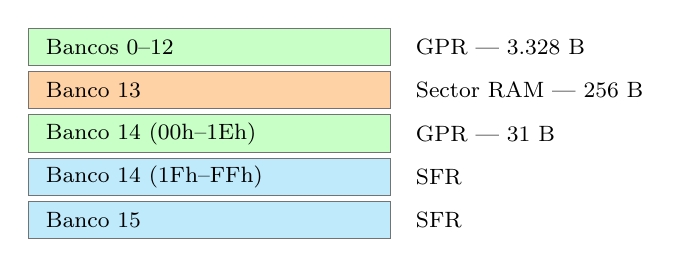
\begin{tikzpicture}[font=\small, y=5.5mm, x=1mm]
    \foreach \i/\et/\col in {
      0/{Bancos 0--12}/{green!22},
      1/{Banco 13}/{orange!35},
      2/{Banco 14 (00h--1Eh)}/{green!22},
      3/{Banco 14 (1Fh--FFh)}/{cyan!25},
      4/{Banco 15}/{cyan!25}}
      {
        \fill[\col, draw=black!55] (0,-\i) rectangle (46,-\i+0.86);
        \node[anchor=west, font=\footnotesize] at (1,-\i+0.43) {\et};
      }
    \node[anchor=west, font=\footnotesize] at (48,0.43)    {GPR — 3.328 B};
    \node[anchor=west, font=\footnotesize] at (48,-1+0.43) {Sector RAM — 256 B};
    \node[anchor=west, font=\footnotesize] at (48,-2+0.43) {GPR — 31 B};
    \node[anchor=west, font=\footnotesize] at (48,-3+0.43) {SFR};
    \node[anchor=west, font=\footnotesize] at (48,-4+0.43) {SFR};
  \end{tikzpicture}
  \caption{Reparto de la memoria de datos del PIC18F47Q10 en bancos
           \cite{microchip2024ds40002043}}
  \label{fig:bancos}
\end{figure}

Los registros de propósito general suman 3.359 bytes utilizables. El banco 13 no
almacena variables: aloja los registros intermedios que participan en la
escritura de la memoria de programa por sectores.

\subsection{Modos de direccionamiento}

La arquitectura ofrece cuatro modos, y la elección entre ellos determina qué
estructuras de datos son expresables con eficiencia.

El direccionamiento \textbf{inherente} corresponde a instrucciones sin operando
explícito. El \textbf{literal} incorpora una constante en la propia instrucción.
El \textbf{directo} codifica los 8 bits bajos de la dirección y obtiene los
4 restantes del registro de selección de banco, salvo que un bit de la
instrucción fuerce el espacio de acceso rápido.

El \textbf{indirecto} emplea tres pares de registros de selección de archivo que
albergan direcciones completas de 12 bits, con los que se alcanza cualquier
banco sin depender del registro de selección. El acceso se realiza a través de
operandos virtuales que, además de leer o escribir, incrementan o decrementan
automáticamente el puntero, o le aplican un desplazamiento con signo. Son estos
operandos los que hacen viables los vectores y las tablas en memoria de datos.

Habilitar el juego de instrucciones extendido añade un quinto modo, indexado con
desplazamiento literal, y \textbf{altera la interpretación del espacio de acceso
rápido}, lo que constituye una de las incompatibilidades más difíciles de
diagnosticar en esta familia.

\subsection{Palabras de configuración}

Seis palabras de 16 bits, grabadas junto al programa a partir de la dirección
\texttt{0x300000}, fijan el comportamiento del dispositivo desde el arranque
\cite{microchip2024ds40002043}. Determinan la fuente de reloj inicial, el
comportamiento del temporizador de guardia, los umbrales de reinicio por caída de
tensión, la protección de las regiones de memoria y la habilitación del juego
extendido.

Su particularidad es que no son modificables en tiempo de ejecución: un valor
equivocado no produce un error de compilación sino un dispositivo que arranca a
una frecuencia distinta de la prevista, o que se reinicia sin causa aparente. Por
tanto, cualquier código de inicialización completo debe incluirlas.

\subsection{Sistema de interrupciones}

El dispositivo atiende las interrupciones mediante dos vectores fijos, situados
en las direcciones \texttt{0x0008} y \texttt{0x0018} de la memoria de programa,
correspondientes a los niveles de prioridad alta y baja
\cite{microchip2024ds40002043}. Cada fuente dispone de un bit de habilitación
individual, un bit indicador de que el suceso se ha producido y un bit que fija
su prioridad, además de dos bits de habilitación global.

Dos particularidades condicionan el código que atiende una interrupción. La
primera es que el indicador no se limpia por hardware al entrar en la rutina:
corresponde al programador borrarlo, y omitirlo provoca que la rutina se invoque
de forma indefinida. La segunda es la conservación del contexto. La arquitectura
dispone de una pila rápida de un solo nivel para tres registros del núcleo, que
se guarda automáticamente al vectorizar; pero si se emplean los dos niveles de
prioridad, una interrupción de prioridad alta que interrumpa a una de baja
sobrescribe esos valores. En ese caso el contexto debe conservarse por software.

Ambas son fuentes de error que no se manifiestan como fallos de compilación sino
como comportamiento errático en ejecución, lo que las hace especialmente
adecuadas para valorar la corrección del código generado.

\subsection{Periféricos independientes del núcleo}

El rasgo distintivo de la familia Q10 es su conjunto de periféricos
independientes del núcleo, capaces de operar sin intervención del procesador. El
dispositivo integra ocho celdas lógicas configurables, dos módulos de captura,
comparación y modulación por ancho de pulso, dos moduladores adicionales de
10 bits, un generador de formas de onda complementarias, cuatro temporizadores
de 16 bits y tres de 8 bits con limitador por hardware, dos transmisores-%
receptores universales síncronos y asíncronos mejorados, y dos puertos serie
síncronos maestros que implementan las interfaces SPI e I\textsuperscript{2}C.

En el apartado analógico destaca el convertidor analógico-digital con
computación: además de la conversión a 10 bits sobre 35 canales externos,
incorpora en hardware el promediado, el filtrado, el sobremuestreo y la
comparación contra umbrales. Completan el conjunto dos comparadores, un
convertidor digital-analógico de 5 bits, una referencia de tensión fija, un
detector de cruce por cero y un detector de tensión alta y baja.

La consecuencia de diseño es relevante para este trabajo: una función que en
otras arquitecturas exigiría atención continua del procesador puede resolverse
configurando registros, con el núcleo detenido. El precio es que la complejidad
se traslada del código a la configuración.

\subsection{Periféricos disponibles}

La tabla \ref{tab:perifericos} recoge el inventario del dispositivo, que fija el
alcance funcional que un sistema generador debe ser capaz de cubrir.

\begin{table}[H]
  \centering
  \caption{Periféricos del PIC18F47Q10 \cite{microchip2024ds40002043}}
  \label{tab:perifericos}
  \begin{tabular}{@{}llr@{}}
    \toprule
    \textbf{Categoría} & \textbf{Módulo} & \textbf{Cantidad} \\
    \midrule
    Temporización & Temporizadores de 16 bits & 4 \\
                  & Temporizadores de 8 bits con limitador & 3 \\
                  & Captura, comparación y modulación & 2 \\
                  & Moduladores de ancho de pulso & 2 \\
    \midrule
    Lógica        & Celdas lógicas configurables & 8 \\
                  & Generador de formas complementarias & 1 \\
                  & Modulador de señal de datos & 1 \\
    \midrule
    Comunicación  & Puertos serie síncronos maestros & 2 \\
                  & Transmisores-receptores universales & 2 \\
    \midrule
    Analógico     & Convertidor analógico-digital con computación & 1 \\
                  & Comparadores & 2 \\
                  & Convertidor digital-analógico de 5 bits & 1 \\
    \bottomrule
  \end{tabular}
\end{table}

La memoria de programa admite escritura desde el propio firmware, lo que
posibilita cargadores de arranque residentes. Su borrado opera por sectores de
128 palabras, y toda operación de escritura exige una secuencia de desbloqueo
que debe ejecutarse sin interrupciones \cite{microchip2024ds40002043}.

\subsection{La configuración de un periférico como problema}

Poner en marcha un periférico en esta familia no se agota en escribir sus
propios registros. Intervienen al menos tres mecanismos transversales que actúan
sobre módulos distintos y que se documentan en secciones alejadas del manual.

El primero es la selección de pines de periférico, que desacopla las señales
digitales de los pines físicos. Una salida no aparece en un pin hasta que se
escribe el registro de asignación correspondiente, y la secuencia de
desbloqueo debe respetarse con exactitud. Un bit de configuración puede además
limitar ese desbloqueo a una sola vez tras el reinicio, de modo que un segundo
intento de remapeo queda sin efecto.

El segundo es la deshabilitación selectiva de módulos, pensada para reducir el
consumo. Un periférico cuyo bit correspondiente esté activo no responde a
ninguna escritura, y el síntoma —un módulo que se configura sin error y no
funciona— no apunta por sí mismo a la causa.

El tercero es el bit que habilita el juego de instrucciones extendido, que
altera la semántica del direccionamiento de datos para todo el programa. La
práctica totalidad del código de ejemplo disponible presupone que está
desactivado, sin declararlo.

A estos se suma el direccionamiento por bancos ya descrito. El resultado es que
un fragmento de código correcto según la sección del periférico puede fallar por
causas descritas doscientas páginas más adelante.

\subsection{La documentación del fabricante como fuente de conocimiento}

La información necesaria para configurar el dispositivo está distribuida en un
conjunto de documentos con distinto alcance y distinta autoridad. El manual
principal describe el comportamiento nominal
\cite{microchip2024ds40002043}; la errata de silicio recoge las desviaciones
observadas en el circuito real y las correcciones al manual, de modo que
\textbf{prevalece sobre él ante cualquier conflicto} \cite{microchip2024errata};
la especificación de programación documenta el acceso de bajo nivel a las
memorias no volátiles \cite{microchip2023progspec}; y las notas de aplicación y
los informes técnicos ilustran usos concretos de cada módulo.

Dos rasgos de este material condicionan el diseño de un sistema de recuperación.
El primero es que el manual cubre simultáneamente varios dispositivos de la
familia, con tablas que los diferencian: una cifra leída sin comprobar la
columna correspondiente puede pertenecer a otro integrado. El segundo es que la
información determinante —mapas de registros, asignación de pines, mapas de
memoria— reside en tablas y figuras, no en prosa continua.

% ===========================================================================
\section{Desarrollo de firmware en C con XC8}
% ===========================================================================

El código que el sistema debe producir se escribe en lenguaje C y se compila con
XC8, el compilador de Microchip para sus microcontroladores de 8 bits
\cite{microchip2012xc8}.

\subsection{Modelo de compilación}

XC8 implementa el estándar C con extensiones específicas para la arquitectura.
La cabecera \texttt{<xc.h>} expone los registros de función especial como
variables y da acceso a sus campos de bits mediante estructuras, de modo que el
código fuente reproduce la nomenclatura del manual. Las directivas
\texttt{\#pragma config} fijan los bits de las palabras de configuración, que se
graban junto al programa y determinan el comportamiento del dispositivo desde el
arranque.

Las rutinas de atención a interrupción se declaran con calificadores propios que
indican su nivel de prioridad. La gestión de la memoria bancada es
responsabilidad del compilador, que inserta las instrucciones de selección de
banco necesarias, pero el programador conserva control sobre la ubicación de las
variables.

La cadena se completa con el entorno de desarrollo integrado y con la placa de
evaluación, cuyo depurador integrado permite programar y depurar el dispositivo
sin instrumental adicional \cite{microchip2020curiosity}.

Al finalizar la compilación, XC8 emite un informe con el consumo de memoria de
programa y de datos. Ese informe es la fuente de los criterios de eficiencia que
se emplean más adelante.

El código \ref{cod:minimo} ilustra la estructura de un programa mínimo. Concentra
los elementos que todo código generado debe incluir: palabras de configuración,
frecuencia del oscilador, inicialización de los registros de dirección y de modo
analógico, y bucle principal.

\begin{lstlisting}[caption={Estructura mínima de un programa para el PIC18F47Q10},
                   label={cod:minimo}]
#include <xc.h>

// Palabras de configuracion: fijan el comportamiento desde el arranque
#pragma config FEXTOSC = OFF     // Sin oscilador externo
#pragma config RSTOSC = HFINTOSC_64MHZ
#pragma config WDTE = OFF        // Temporizador de guardia deshabilitado
#pragma config XINST = OFF       // Juego extendido desactivado

#define _XTAL_FREQ 64000000UL    // Requerido por las rutinas de retardo

void main(void)
{
    ANSELDbits.ANSELD0 = 0;      // RD0 en modo digital, no analogico
    TRISDbits.TRISD0   = 0;      // RD0 como salida

    while (1) {
        LATDbits.LATD0 ^= 1;     // Conmuta el nivel del pin
        __delay_ms(500);
    }
}
\end{lstlisting}

Obsérvese que la asignación del modo analógico precede a la de dirección: los
pines con capacidad analógica arrancan en ese modo, de manera que omitir esa
línea produce un programa que compila y no conmuta el pin. Es un ejemplo del tipo
de conocimiento tácito que un sistema generador debe incorporar.

\subsection{Gestión de la memoria bancada}

La memoria de datos en bancos, descrita en la sección anterior, plantea al
compilador una decisión que el lenguaje C no expresa: dónde ubicar cada variable
y cuándo conmutar de banco. XC8 la resuelve automáticamente, insertando las
instrucciones de selección necesarias y agrupando las variables para minimizar
el número de conmutaciones.

El programador conserva, no obstante, mecanismos para intervenir. Puede solicitar
que una variable resida en el espacio de acceso rápido, con lo que se alcanza en
un solo ciclo sin conmutar de banco, o fijarla en una dirección concreta. Ambas
posibilidades importan cuando se compara la eficiencia de realizaciones
distintas de una misma funcionalidad, porque una diferencia en el consumo de
memoria de datos puede deberse tanto al algoritmo como a estas decisiones de
ubicación.

\subsection{Generación de configuraciones con MCC}

El configurador de código de MPLAB, conocido por sus siglas en inglés MCC
(\emph{MPLAB Code Configurator}), permite describir gráficamente la
configuración de los periféricos y generar a partir de ella el código de
inicialización. Guarda esa descripción en un archivo propio con extensión
\texttt{.mc3}, separado del código que produce
\cite{microchip2022mcc}.

La herramienta admite varias modalidades de contenido \cite{microchip2022mcc},
y en este trabajo intervienen dos con papeles distintos. Los proyectos de ejemplo
publicados por el fabricante están generados con \emph{MCC Classic} y se emplean
como corpus de contraste; los proyectos propios, de los que sale el patrón de
referencia, se generan con \emph{MCC Melody}, la única modalidad que ofrece la
extensión de MPLAB para Visual Studio Code. La distinción no es accesoria: cada
modalidad genera código con una estructura distinta, de modo que la comparación
estructural de un archivo generado solo tiene sentido dentro de la misma
modalidad. Por esa razón la fidelidad se contrasta sobre los valores escritos en
los registros de configuración, que no dependen de la modalidad que los produjo.

Esta separación entre especificación y código resulta de interés metodológico:
cada proyecto generado con MCC constituye un par formado por una especificación
declarativa y el código que el fabricante considera su realización correcta. Ese
par ofrece un patrón de referencia natural frente al cual contrastar el código
que produzca un sistema automático.

\subsection{Criterios de eficiencia}

La evaluación de un firmware no se agota en su corrección funcional. En un
dispositivo con 128\,KB de memoria de programa y algo menos de 3,3\,KB
utilizables de memoria de datos, el consumo de recursos es una restricción de
diseño. Se adoptan como métricas los bytes ocupados en cada una de esas
memorias, tomados del informe del compilador, lo que permite comparar
realizaciones distintas de una misma funcionalidad.

% ===========================================================================
\section{Modelos de lenguaje de gran escala y generación de código}
% ===========================================================================

Un modelo de lenguaje de gran escala, designado habitualmente por sus siglas en
inglés LLM (\emph{Large Language Model}), es una red neuronal entrenada para
estimar la probabilidad del siguiente elemento de una secuencia de texto. Su
aplicación a la generación de código explota el hecho de que un programa es,
formalmente, una secuencia de símbolos con regularidades estadísticas.

\subsection{La arquitectura Transformer}

Los modelos actuales derivan de la arquitectura Transformer, que prescinde de la
recurrencia y de la convolución y basa el procesamiento exclusivamente en
mecanismos de atención \cite{vaswani2017attention}. La atención pondera la
relevancia de cada elemento de la secuencia respecto de los demás, lo que
permite capturar dependencias entre posiciones alejadas sin recorrer las
intermedias.

Su ventaja decisiva es la paralelización: al no existir dependencia secuencial
entre posiciones, el entrenamiento aprovecha el cómputo paralelo, lo que hizo
viable escalar tanto el tamaño de los modelos como el de los corpus.

Formalmente, la atención opera sobre tres proyecciones de la secuencia de
entrada —consultas $Q$, claves $K$ y valores $V$— y se calcula como

\begin{equation}
  \mathrm{Atenci\acute{o}n}(Q,K,V) = \mathrm{softmax}\!\left(
    \frac{QK^{\mathsf{T}}}{\sqrt{d_k}} \right) V ,
  \label{eq:atencion}
\end{equation}

donde $d_k$ es la dimensión de las claves y el factor $1/\sqrt{d_k}$ evita que el
producto escalar crezca hasta saturar la función exponencial
\cite{vaswani2017attention}. El modelo aplica varias de estas operaciones en
paralelo, cada una con proyecciones distintas, lo que le permite atender
simultáneamente a relaciones de naturaleza diferente.

\subsection{Tokenización y ventana de contexto}

El texto no se procesa carácter a carácter sino en unidades denominadas
\emph{tokens}, obtenidas por un algoritmo de segmentación subléxica. Un modelo
solo puede atender a un número acotado de \emph{tokens} simultáneamente: es la
llamada ventana de contexto.

Esta limitación es central para este trabajo. El manual del dispositivo supera
las setecientas páginas, de modo que no cabe íntegro en la ventana de contexto
de los modelos de uso corriente. Aun cuando cupiera, la evidencia experimental
muestra que la capacidad de un modelo para utilizar la información degrada con
la longitud del contexto, y que los elementos situados en posiciones centrales
se aprovechan peor que los de los extremos \cite{liu2024lost}.

La segmentación subléxica tiene una consecuencia directa en este dominio. Un
identificador como \texttt{ANSELDbits} no constituye una unidad para el modelo,
sino que se fragmenta en varias piezas según su frecuencia en el corpus. Cuanto
más raro sea el término, en más piezas se divide y menor es la evidencia
estadística de que dispone el modelo para reproducirlo con exactitud.

\subsection{Estrategias de decodificación}

Un modelo no emite un símbolo determinado sino una distribución de probabilidad
sobre el vocabulario, y la estrategia de decodificación decide cómo obtener de
ella la salida. La selección voraz toma en cada paso el elemento más probable y
produce resultados reproducibles. El muestreo introduce aleatoriedad controlada
por un parámetro de temperatura: valores bajos concentran la probabilidad en los
candidatos dominantes y valores altos la reparten.

Esta elección afecta a la evaluación. Una temperatura no nula hace que dos
ejecuciones con la misma entrada produzcan salidas distintas, de modo que
cualquier métrica debe calcularse sobre varias muestras y acompañarse del
parámetro empleado. La métrica \emph{pass@k} presupone precisamente ese
muestreo repetido \cite{chen2021codex}.

\subsection{Generación de código y su evaluación}

El trabajo que estableció el marco de evaluación hoy dominante presentó un
modelo entrenado específicamente sobre código junto con un conjunto de problemas
de programación y una métrica asociada \cite{chen2021codex}. Esa métrica,
denominada \emph{pass@k}, estima la probabilidad de que al menos una de $k$
muestras generadas supere las pruebas del problema.

Su interés radica en que evalúa el comportamiento del código, no su parecido con
una solución de referencia. Un programa puede resolver correctamente un problema
con una redacción muy distinta de la esperada, y las métricas basadas en
similitud textual lo penalizarían.

\subsection{Instrucciones de sistema}

Además de la consulta, el modelo recibe un texto que fija su comportamiento: el
papel que adopta, el formato de la respuesta y las restricciones que debe
respetar. En un sistema de generación de firmware, ese texto es el lugar donde
se imponen la nomenclatura exacta de los registros, el estilo de código del
compilador y la obligación de citar la sección del manual que respalda cada
decisión. Su redacción constituye, por tanto, una decisión de diseño y no un
detalle de implementación.

\subsection{Limitaciones}

Tres limitaciones condicionan el empleo directo de estos modelos en el dominio
que ocupa a este trabajo.

La primera es la generación de contenido incorrecto con apariencia plausible.
Un modelo puede producir nombres de registro inexistentes o campos de bits con
anchura equivocada, y presentarlos con la misma seguridad que los correctos.

La segunda es el corte de conocimiento: el modelo solo dispone de lo que estaba
en su corpus de entrenamiento, sin acceso a documentación posterior ni a
erratas.

La tercera, específica del dominio, es la escasez de vocabulario especializado.
Los nombres de registro, los prefijos de fabricante y las constantes de hardware
aparecen con muy baja frecuencia en corpus generalistas, de modo que el modelo
dispone de poca evidencia estadística sobre ellos.

\subsection{Antecedentes en sistemas embebidos}

La literatura reciente ha caracterizado experimentalmente estas capacidades y
límites. Un estudio sobre desarrollo y depuración de sistemas empotrados
concluye que los modelos actuales alcanzan un grado notable de razonamiento
entre dominios, generando controladores a nivel de registro y código de
comunicación funcional, y que incluso cuando el código resultante no es correcto
el razonamiento que lo acompaña resulta de utilidad \cite{englhardt2023embedded}.
El mismo trabajo observa que parte del conocimiento del modelo sobre el hardware
procede de la presencia de hojas de datos en su corpus de entrenamiento, y que
suministrarle una representación legible de los registros relevantes mejora
sustancialmente el resultado.

Esta observación es precisamente la hipótesis de la que parte el presente
proyecto. En la misma línea, un trabajo posterior aplica recuperación de
información a la generación de capas de abstracción de hardware para
microcontroladores de otro fabricante, integrándola en el flujo de desarrollo
existente \cite{haug2025microcontrollers}. Ambos antecedentes delimitan el
espacio en que se sitúa esta pasantía: la técnica está validada, y lo que se
aporta es su realización sobre la familia PIC18-Q10 y su cadena de herramientas,
con un ciclo de validación basado en compilación.

% ===========================================================================
\section{Generación aumentada por recuperación}
% ===========================================================================

La generación aumentada por recuperación, conocida por sus siglas en inglés RAG
(\emph{Retrieval-Augmented Generation}), combina un modelo de lenguaje con un
sistema de recuperación de información sobre un corpus externo
\cite{lewis2020rag}. En lugar de responder únicamente con el conocimiento
almacenado en sus parámetros, el modelo recibe junto a la consulta un conjunto
de fragmentos recuperados del corpus y genera a partir de ellos.

\subsection{Fundamento}

La formulación original distingue dos tipos de memoria. La memoria paramétrica
es el conocimiento codificado en los pesos durante el entrenamiento: extenso
pero difuso, imposible de inspeccionar y costoso de actualizar. La memoria no
paramétrica es un índice sobre documentos, consultable en tiempo de inferencia y
modificable sin reentrenar \cite{lewis2020rag}.

Para el problema que ocupa a este trabajo, esa distinción resuelve tres
dificultades simultáneamente. La documentación del dispositivo puede
actualizarse sin tocar el modelo; la respuesta queda anclada a un fragmento
concreto y, por tanto, es verificable; y la escasez de vocabulario especializado
en el corpus de entrenamiento deja de ser determinante, porque los nombres de
registro llegan al modelo en el propio contexto.

\subsection{Arquitectura}

Un sistema RAG opera en tres etapas, representadas en la figura
\ref{fig:arquitectura-rag}. La indexación se ejecuta una sola vez, mientras que
la recuperación y la generación se ejecutan en cada consulta.

\begin{figure}[H]
  \centering
  \begin{tikzpicture}[
      font=\small,
      caja/.style={draw, rounded corners=2pt, minimum height=8mm,
                   minimum width=22mm, align=center, inner sep=3pt},
      docu/.style={caja, fill=gray!8},
      proc/.style={caja, fill=blue!6},
      flecha/.style={-{Stealth[length=2mm]}, thick}
    ]
    % Indexación
    \node[docu] (corpus) {Corpus\\documental};
    \node[proc, right=7mm of corpus] (seg) {Segmen-\\tación};
    \node[proc, right=7mm of seg] (emb) {Vectori-\\zación};
    \node[docu, right=7mm of emb] (idx) {Índice\\vectorial};
    \draw[flecha] (corpus) -- (seg);
    \draw[flecha] (seg) -- (emb);
    \draw[flecha] (emb) -- (idx);
    \node[above=1mm of seg, font=\small\itshape] {Indexación (una vez)};

    % Consulta
    \node[docu, below=14mm of corpus] (query) {Consulta};
    \node[proc, below=14mm of seg] (rec) {Recupe-\\ración};
    \node[proc, below=14mm of emb] (ctx) {Contexto\\+ consulta};
    \node[proc, below=14mm of idx] (llm) {Modelo de\\lenguaje};
    \node[docu, below=8mm of llm] (out) {Código\\generado};
    \draw[flecha] (query) -- (rec);
    \draw[flecha] (rec) -- (ctx);
    \draw[flecha] (ctx) -- (llm);
    \draw[flecha] (llm) -- (out);
    \draw[flecha] (idx) -- (rec.north east) node[midway, right, font=\scriptsize] {};
    \node[below=1mm of rec, font=\small\itshape, yshift=-6mm] {Recuperación y generación (por consulta)};
  \end{tikzpicture}
  \caption{Etapas de un sistema de generación aumentada por recuperación}
  \label{fig:arquitectura-rag}
\end{figure}

\subsection{Extracción de documentación técnica}

Antes de segmentar hay que convertir el documento a texto, y en formatos
paginados esa conversión no es neutra. Un extractor orientado a prosa recorre el
contenido en orden de lectura y produce una secuencia plana, con lo que la
información dispuesta en dos dimensiones se pierde.

El efecto sobre el material de este proyecto es directo. Un mapa de registros
presenta en columnas la dirección, el nombre y los campos de bits; leído como
texto plano, esas columnas se entremezclan y el resultado es inservible.
Conservar la alineación mediante las opciones adecuadas del extractor mantiene
la tabla legible, pero no todos los elementos sobreviven: los mapas de memoria,
los diagramas de bloques y los esquemas de pines son figuras, y de ellos no
queda nada. Tampoco sobrevive el sombreado con que algunas tablas distinguen a
qué dispositivo aplica cada fila.

De ahí que la elección de la herramienta de extracción no sea un detalle de
implementación sino una decisión que condiciona la calidad de todo el corpus.
Las alternativas van desde los extractores de texto tradicionales hasta los
sistemas que reconstruyen la estructura del documento y representan las tablas
como tales. Cuando un dato depende de una figura, la única vía es interpretarla
como imagen o transcribirla manualmente.

\subsection{Segmentación del corpus}

Los documentos no se indexan enteros sino divididos en fragmentos. El tamaño del
fragmento establece un compromiso: uno demasiado extenso diluye la señal de
relevancia e introduce ruido en el contexto; uno demasiado breve pierde la
información necesaria para interpretarlo.

En documentación técnica esta decisión adquiere una dificultad añadida. Una
tabla de registros separada de su encabezado pierde el significado de sus
columnas, y una cifra separada de la nota al pie que la matiza puede inducir a
error. El manual del dispositivo contiene ejemplos de ambas situaciones
\cite{microchip2024ds40002043}. La estrategia de segmentación debe, por tanto,
preservar la unidad entre una tabla, su título y sus notas.

Se distinguen tres familias de estrategias. La segmentación por \textbf{tamaño
fijo} divide el texto en bloques de longitud constante, habitualmente con
solapamiento entre bloques consecutivos para no partir una idea por la mitad; es
simple pero ignora la estructura del documento. La segmentación \textbf{por
estructura} aprovecha la jerarquía de secciones y subsecciones, de modo que cada
fragmento coincide con una unidad lógica. La segmentación \textbf{semántica}
decide los cortes según la afinidad entre pasajes contiguos.

Para documentación técnica, la segunda resulta la más adecuada, porque la
jerarquía del manual ya refleja la organización del conocimiento. Requiere, eso
sí, una extracción del documento que conserve esa jerarquía, lo que en formatos
paginados no es inmediato.

\subsection{Metadatos y filtrado}

Cada fragmento puede acompañarse de atributos que no participan en la
comparación vectorial pero permiten restringir la búsqueda: el documento de
origen, la sección, la página, el periférico tratado o el dispositivo al que
aplica.

Este último resulta indispensable en el caso que ocupa a este trabajo. Dado que
el manual describe simultáneamente dos dispositivos de la familia
\cite{microchip2024ds40002043}, un fragmento recuperado sin filtrar por
dispositivo puede contener cifras que no corresponden al integrado empleado. El
filtrado por metadatos convierte esa distinción en una restricción explícita de
la consulta en lugar de dejarla al criterio del modelo.

\subsection{Representación vectorial y búsqueda densa}

La recuperación densa representa fragmentos y consultas como vectores en un
espacio de dimensión fija, de modo que la proximidad geométrica aproxime la
afinidad semántica \cite{karpukhin2020dpr}. La consulta se vectoriza con el
mismo procedimiento y se recuperan los $k$ fragmentos más próximos según una
medida de similitud, habitualmente el coseno del ángulo entre vectores.

La obtención de representaciones adecuadas para comparar textos completos exigió
adaptaciones específicas sobre los modelos de lenguaje preexistentes, ya que
estos no producían de forma nativa vectores comparables mediante similitud
\cite{reimers2019sbert}.

La proximidad entre vectores se cuantifica habitualmente mediante la similitud
del coseno, que para dos vectores $\mathbf{u}$ y $\mathbf{v}$ se define como

\begin{equation}
  \mathrm{sim}(\mathbf{u},\mathbf{v}) =
    \frac{\mathbf{u} \cdot \mathbf{v}}
         {\lVert \mathbf{u} \rVert \, \lVert \mathbf{v} \rVert} .
  \label{eq:coseno}
\end{equation}

Su interés reside en que atiende únicamente a la orientación de los vectores y
no a su magnitud, de modo que un fragmento extenso y otro breve que traten el
mismo asunto resultan igualmente próximos a la consulta.

La ventaja de este enfoque es que reconoce equivalencias semánticas sin
coincidencia literal. Su limitación aparece precisamente en el dominio de este
trabajo: un identificador como \texttt{TRISD} o \texttt{PPS1WAY} carece de
sinónimos, y lo que interesa de él es su aparición exacta.

\subsection{Recuperación cruzada entre idiomas}

La documentación del fabricante está escrita en inglés y las peticiones al
sistema se formulan en español. La recuperación es, por tanto, cruzada entre
idiomas por diseño, y esa condición impone un requisito sobre la
representación vectorial que conviene establecer antes de elegir el modelo que
la produce.

Un modelo entrenado sobre un solo idioma no dispone de ningún mecanismo que
acerque una expresión a su traducción. La consulta \emph{«configurar el
conversor analógico-digital»} y el fragmento \emph{«ADC with Computation»}
designan lo mismo, pero un codificador monolingüe los sitúa en regiones
distintas del espacio: la proximidad geométrica que la ecuación
\eqref{eq:coseno} mide deja de aproximar la afinidad semántica en cuanto los
dos textos no comparten idioma.

Los modelos multilingües alineados resuelven esa separación construyendo un
espacio común. El procedimiento de destilación de conocimiento propuesto por
Reimers y Gurevych entrena un modelo alumno para que sitúe una frase traducida
\emph{en el mismo lugar} que ocupa la original en el espacio del modelo
maestro, de modo que la equivalencia entre idiomas queda codificada en la
geometría y no delegada a una traducción previa
\cite{reimers2020multilingual}. El alineamiento entre idiomas admite además
otras familias de métodos, y su alcance y sus límites han sido sistematizados
recientemente \cite{hammerl2024alignment}.

La consecuencia práctica para este trabajo no es la pérdida de calidad en sí,
sino su carácter silencioso. Un recuperador mal alineado no falla: devuelve los
$k$ fragmentos solicitados, formalmente correctos, simplemente peores. No hay
excepción, ni aviso, ni indicio en la respuesta generada de que el contexto
entregado no era el pertinente. Por eso el alineamiento entre idiomas no puede
suponerse a partir de la descripción del modelo y debe verificarse
experimentalmente sobre el corpus del problema, lo que se aborda en el capítulo
siguiente.

\subsection{Búsqueda léxica y estrategias híbridas}

Frente a la anterior, la recuperación léxica puntúa los fragmentos según la
coincidencia de términos, ponderando su frecuencia en el documento y su rareza
en la colección. La formulación de referencia es BM25, dentro del marco
probabilístico de relevancia \cite{robertson2009bm25}.

Las dos aproximaciones son complementarias: la densa capta la intención de la
consulta y la léxica garantiza que un identificador exacto no se pierda. Las
estrategias híbridas combinan ambas puntuaciones, lo que resulta especialmente
pertinente cuando el corpus está poblado de nomenclatura literal.

La combinación no es inmediata, porque las dos puntuaciones no comparten escala.
Un procedimiento habitual prescinde de los valores y opera sobre las posiciones:
la fusión recíproca de rangos asigna a cada fragmento una puntuación

\begin{equation}
  s(d) = \sum_{i} \frac{1}{c + r_i(d)} ,
  \label{eq:rrf}
\end{equation}

donde $r_i(d)$ es la posición del fragmento $d$ en la lista $i$ y $c$ una
constante que atenúa el peso de las primeras posiciones. Al depender solo del
orden, evita tener que normalizar puntuaciones heterogéneas.

\subsection{Índices aproximados}

Comparar la consulta con todos los vectores del índice resulta inviable cuando
este crece. Los índices de vecinos aproximados sacrifican la garantía de
encontrar el óptimo exacto a cambio de una reducción drástica del tiempo de
búsqueda. La estructura más extendida organiza los vectores en un grafo
jerárquico navegable, en el que la búsqueda desciende por capas de densidad
creciente \cite{malkov2020hnsw}.

\subsection{Bases de datos vectoriales}

El almacenamiento de los vectores y sus metadatos, junto con el índice que los
recorre, corresponde a una base de datos vectorial. Frente a una realización
propia sobre una biblioteca de índices, estos sistemas aportan persistencia,
filtrado por metadatos integrado en la búsqueda, actualización incremental del
índice y control de versiones de la colección.

Esa integración importa: filtrar después de recuperar puede dejar menos de $k$
resultados válidos, mientras que hacerlo durante el recorrido del índice
garantiza que los $k$ devueltos cumplen la restricción.

\subsection{Reordenamiento}

La recuperación inicial prioriza el recorrido rápido de un índice extenso, lo
que obliga a comparar consulta y fragmento por separado. Una segunda etapa puede
reordenar un conjunto reducido de candidatos evaluándolos conjuntamente con la
consulta, lo que mejora la precisión a costa de un cómputo mayor
\cite{nogueira2019passage}. Existen formulaciones intermedias que retrasan la
interacción entre ambos textos para conservar parte de esa precisión sin renunciar
a la eficiencia \cite{khattab2020colbert}.

\subsection{Construcción del contexto}

Los fragmentos recuperados se incorporan al contexto junto con la consulta y las
instrucciones de sistema. Dado que el aprovechamiento del contexto no es
uniforme a lo largo de su extensión \cite{liu2024lost}, tanto el número de
fragmentos como su orden constituyen decisiones de diseño con efecto medible
sobre el resultado.

\subsection{Recuperación frente a ajuste fino}

La alternativa a la recuperación es el ajuste fino, esto es, continuar el
entrenamiento del modelo sobre el corpus del dominio para incorporarlo a sus
parámetros. La tabla \ref{tab:ragvsft} contrasta ambas opciones en los aspectos
determinantes para este proyecto.

\begin{table}[H]
  \centering
  \caption{Recuperación aumentada frente a ajuste fino}
  \label{tab:ragvsft}
  \begin{tabular}{@{}p{0.26\textwidth}p{0.33\textwidth}p{0.33\textwidth}@{}}
    \toprule
    \textbf{Aspecto} & \textbf{Recuperación aumentada} & \textbf{Ajuste fino} \\
    \midrule
    Actualización del conocimiento & Reindexar el corpus & Reentrenar el modelo \\
    Trazabilidad de la respuesta & El fragmento citado es verificable & El origen no es inspeccionable \\
    Coste computacional & Indexación y búsqueda & Entrenamiento sobre acelerador \\
    Volumen de datos exigido & Los documentos disponibles & Muchos ejemplos etiquetados \\
    Jerarquía entre fuentes & Se impone al recuperar & Se diluye en los pesos \\
    \bottomrule
  \end{tabular}
\end{table}

La última fila resulta determinante en este dominio. La errata de silicio
corrige al manual y debe prevalecer sobre él \cite{microchip2024errata}. Un
sistema de recuperación puede imponer esa jerarquía de forma explícita; un
modelo ajustado sobre ambos documentos los mezcla en sus parámetros sin
conservar la relación de precedencia. A ello se añade que el volumen documental
disponible —un manual, una errata y un conjunto de notas de aplicación— es
adecuado para construir un índice, pero insuficiente para un entrenamiento.

\subsection{Variantes}

Sobre la formulación básica se han propuesto extensiones. Algunas incorporan al
modelo la decisión de cuándo recuperar y la evaluación crítica de lo recuperado
\cite{asai2024selfrag}. Otras añaden una etapa correctiva que detecta
recuperaciones de baja calidad y actúa en consecuencia \cite{yan2024crag}. Una
tercera línea construye un grafo de entidades y relaciones sobre el corpus para
responder consultas que exigen agregar información dispersa \cite{edge2024graphrag}.

% ===========================================================================
\section{Exposición del sistema mediante el Model Context Protocol}
% ===========================================================================

Un sistema de recuperación resuelve qué fragmentos entregar al modelo, pero no
cómo hacérselos llegar. Históricamente esa unión se resolvía de forma
particular para cada pareja de aplicación y fuente de datos, lo que multiplica
las integraciones: $N$ aplicaciones frente a $M$ fuentes exigen $N \times M$
adaptadores. El \emph{Model Context Protocol} (MCP) es una especificación
abierta que normaliza esa frontera, de modo que cualquier cliente compatible
pueda consumir cualquier servidor compatible \cite{mcp2026spec}.

Para este trabajo la elección no es accesoria. El sistema de recuperación
construido sobre el corpus del PIC18F47Q10 se expone como un servidor MCP, y
con ello queda disponible para cualquier asistente que hable el protocolo sin
reescribir la integración. Esa separación entre el recuperador y el modelo que
lo consume es además lo que permite comparar el desempeño con y sin
recuperación, que es el diseño experimental descrito en la sección siguiente.

\subsection{Arquitectura y capas}

El protocolo distingue tres participantes. El \emph{host} es la aplicación que
coordina —el asistente que el usuario maneja—; el \emph{cliente} es el
componente que mantiene la conexión, y el \emph{servidor} es el proceso que
expone las capacidades. La especificación fija una relación uno a uno entre
cliente y servidor: el host instancia un cliente por cada servidor al que se
conecta, lo que aísla los fallos y delimita los permisos de cada fuente
\cite{mcp2026spec}.

Sobre esa disposición se definen dos capas. La capa de datos establece el
intercambio mediante JSON-RPC 2.0 y comprende el ciclo de vida de la conexión,
el descubrimiento de capacidades y las notificaciones. La capa de transporte
determina el canal físico —entrada y salida estándar para servidores locales,
HTTP para los remotos— y es independiente de la anterior, de manera que un
mismo servidor puede exponerse por cualquiera de las dos sin modificar su
lógica \cite{mcp2026spec}.

\subsection{Primitivas y control}

El servidor expone tres tipos de capacidad, y lo que las distingue no es su
contenido sino quién decide invocarlas. Las \emph{herramientas}
(\emph{tools}) las elige el modelo durante la generación; los \emph{recursos}
(\emph{resources}) los selecciona la aplicación anfitriona; y las
\emph{plantillas de instrucciones} (\emph{prompts}) las invoca el usuario de
forma explícita \cite{mcp2026spec}.

Esa asignación de control importa para el diseño del recuperador. Una consulta
al corpus del microcontrolador debe poder originarse en el propio modelo cuando
detecta que le falta información sobre un registro, lo que la sitúa
naturalmente como herramienta y no como recurso.

\subsection{Estado de la especificación}

MCP es una especificación viva y sus revisiones se identifican por fecha. La
versión vigente durante el desarrollo de este trabajo es \texttt{2026-07-28}
\cite{mcp2026spec}. Conviene señalar que dos primitivas del cliente presentes en
revisiones anteriores —el muestreo (\emph{sampling}) y el registro
(\emph{logging})— quedaron obsoletas en esa revisión, circunstancia que invalida
buena parte del material divulgativo publicado con anterioridad y que obliga a
contrastar cualquier ejemplo contra la especificación vigente.

\section{Evaluación de sistemas de generación de código}
% ===========================================================================

La evaluación debe abarcar dos componentes con modos de fallo distintos: el
recuperador, que puede devolver fragmentos irrelevantes, y el generador, que
puede producir código incorrecto a partir de fragmentos adecuados. Medirlos por
separado permite atribuir los fallos.

\subsection{Métricas sobre el código generado}

La métrica de referencia en generación de código estima la probabilidad de que
al menos una de $k$ muestras supere un conjunto de pruebas \cite{chen2021codex}.
Si de un problema se generan $n$ muestras de las que $c$ resultan correctas, el
estimador insesgado es

\begin{equation}
  \text{\emph{pass@k}} = \mathbb{E}\left[\,
    1 - \frac{\binom{n-c}{k}}{\binom{n}{k}} \right] ,
  \label{eq:passk}
\end{equation}

expresión que evita la varianza elevada que tendría el cálculo directo sobre $k$
muestras \cite{chen2021codex}.
Su aplicación a firmware presenta una particularidad: ejecutar el código exige
el dispositivo o un simulador, lo que encarece la evaluación.

Por ello se adopta como criterio primario la \textbf{tasa de compilación
exitosa}: la proporción de generaciones que el compilador acepta sin errores.
Es un criterio necesario aunque no suficiente —un programa puede compilar y no
funcionar—, pero resulta objetivo, automatizable y sensible a los errores
característicos del dominio, como un nombre de registro inexistente.

A ella se añaden dos criterios complementarios. La \textbf{fidelidad a la
configuración de referencia} compara, registro a registro, el código generado
con el que produce la herramienta del fabricante para la misma especificación.
La \textbf{eficiencia en recursos} contrasta el consumo de memoria de programa y
de datos frente a los umbrales establecidos.

\subsection{Evaluación del recuperador}

El recuperador se evalúa con las métricas propias de la recuperación de
información, sobre un conjunto de consultas con su respuesta esperada. La
cobertura entre los $k$ primeros resultados mide si el fragmento pertinente
llegó a recuperarse; el rango recíproco medio pondera además la posición en que
lo hizo.

Medir esta etapa de forma aislada es metodológicamente necesario: si el
fragmento correcto no se recupera, ninguna mejora en el generador puede
compensarlo, y una evaluación conjunta no distinguiría ambas causas. Existen
marcos que automatizan la valoración conjunta del sistema
\cite{es2024ragas}, útiles como complemento pero no como sustituto de la medida
por etapas.

\subsection{Validación automática con realimentación}

El compilador no solo dictamina si el código es aceptable: emite diagnósticos
que localizan el error y lo describen. Esa información puede reinyectarse al
modelo para que corrija su propia salida, según el ciclo de la figura
\ref{fig:ciclo-validacion}.

\begin{figure}[H]
  \centering
  \begin{tikzpicture}[
      font=\small,
      caja/.style={draw, rounded corners=2pt, minimum height=8mm,
                   minimum width=24mm, align=center, inner sep=3pt, fill=blue!6},
      dec/.style={draw, diamond, aspect=2.2, align=center, inner sep=1pt,
                  fill=gray!8, minimum height=8mm},
      flecha/.style={-{Stealth[length=2mm]}, thick}
    ]
    \node[caja] (gen) {Generación};
    \node[caja, right=10mm of gen] (comp) {Compilación};
    \node[dec, right=10mm of comp] (ok) {¿Errores?};
    \node[caja, right=10mm of ok] (fin) {Código\\validado};
    \draw[flecha] (gen) -- (comp);
    \draw[flecha] (comp) -- (ok);
    \draw[flecha] (ok) -- node[above, font=\scriptsize] {no} (fin);
    \draw[flecha] (ok.south) -- ++(0,-9mm) -| node[pos=0.25, below, font=\scriptsize]
      {sí: diagnósticos del compilador} (gen.south);
  \end{tikzpicture}
  \caption{Ciclo de validación con realimentación de errores}
  \label{fig:ciclo-validacion}
\end{figure}

El ciclo exige fijar dos parámetros: el número máximo de iteraciones antes de
declarar el fallo y el criterio de convergencia. Ambos condicionan los
resultados y deben declararse explícitamente al presentarlos, ya que la tasa de
éxito con corrección iterativa no es comparable con la obtenida en un solo
intento.

\subsection{Diseño experimental}

La afirmación central de este trabajo es que la recuperación mejora la calidad
del código generado. Contrastarla exige un experimento de ablación en el que la
presencia del sistema de recuperación sea la única variable: mismo modelo,
mismas consultas, mismas instrucciones de sistema y mismos criterios de medida.
Cualquier otra diferencia entre ambas condiciones comprometería la atribución
del efecto observado.

Dos precauciones de orden estadístico acompañan a ese diseño. La primera es el
tamaño del conjunto de consultas: una diferencia entre condiciones solo resulta
interpretable si el número de casos permite distinguirla de la variabilidad
propia del muestreo. La segunda es que, con temperatura no nula, cada consulta
debe repetirse varias veces y las métricas calcularse sobre el conjunto,
declarando tanto el número de repeticiones como el valor del parámetro.

La tabla \ref{tab:metricas} resume el conjunto de medidas y el componente que
evalúa cada una.

\begin{table}[H]
  \centering
  \caption{Métricas de evaluación y componente evaluado}
  \label{tab:metricas}
  \begin{tabular}{@{}llp{0.42\textwidth}@{}}
    \toprule
    \textbf{Métrica} & \textbf{Componente} & \textbf{Qué mide} \\
    \midrule
    \emph{recall@k} & Recuperador & Si el fragmento pertinente se recupera \\
    MRR & Recuperador & En qué posición lo hace \\
    Tasa de compilación & Generador & Proporción de código que el compilador acepta \\
    Fidelidad & Generador & Coincidencia registro a registro con la referencia \\
    Eficiencia & Generador & Memoria de programa y de datos consumida \\
    \emph{pass@k} & Generador & Probabilidad de acierto en $k$ intentos \\
    \bottomrule
  \end{tabular}
\end{table}
